% !TEX program = xelatex
% basic document config
\documentclass[a4paper,10pt,xetex]{article}
\usepackage[a4paper,top=45mm,right=20mm,bottom=30mm,left=25mm,head=35mm,foot=20mm]{geometry}

% language
\usepackage[german]{babel}

% variable definitions
\providecommand{\documenttitle}{Bedienungsanleitung}
\providecommand{\documentauthors}{Andreas Saurer \\ Benjamin Schneidinger \\ Josef Erben \\ Raffaele Bof \\ Nicolas Loth}
\providecommand{\documentdate}{16.05.2017}
\providecommand{\documentversion}{1.0.0}

% special commands
\newcommand*{\fullref}[1]{\hyperref[{#1}]{\nameref*{#1} (\ref*{#1})}}
\newcommand{\specialcell}[2][c]{%
  \begin{tabular}[#1]{@{}l@{}}#2\end{tabular}}

% font
% \usepackage{titling}
\usepackage[sfdefault]{roboto}
\usepackage[parfill]{parskip}
\usepackage{soul}

% table
\usepackage{array}
\usepackage{multicol}
\usepackage{longtable,tabu,booktabs}

% links
\usepackage{hyperref}
\hypersetup{
            pdftitle={\documenttitle},
            pdfauthor={\documentauthors},
            colorlinks=true,
            linkcolor=[RGB]{74,144,226},
            citecolor=[RGB]{74,144,226},
            urlcolor=[RGB]{74,144,226},
            breaklinks=true}
\urlstyle{same}  % don't use monospace font for urls

% images
\usepackage[font=small,skip=6pt]{caption}
\usepackage{float,graphicx,grffile,wrapfig}
\graphicspath{ {images/} }

\makeatletter
\def\maxwidth{\ifdim\Gin@nat@width>\linewidth\linewidth\else\Gin@nat@width\fi}
\def\maxheight{\ifdim\Gin@nat@height>\textheight\textheight\else\Gin@nat@height\fi}
\makeatother
\setkeys{Gin}{width=\maxwidth,height=\maxheight,keepaspectratio}

\makeatletter
\def\fps@figure{H}
\makeatother

% header and footer
\usepackage{lastpage}
\usepackage{fancyhdr}
\pagestyle{fancy}
\fancyhf{}
\fancyhead[L]{
\includegraphics[height=2cm]{travel-buddy_white}}
\fancyfoot[L]{\fontsize{8}{10}\selectfont\ \documenttitle}
\fancyfoot[R]{\fontsize{8}{10}\selectfont\ Seite\ \thepage\ von\ \pageref*{LastPage}}

\renewcommand{\headrulewidth}{0pt}
\renewcommand{\footrulewidth}{0pt}

% style titles
\usepackage{titlesec}
\titlespacing*{\section}{0pt}{1em}{0pt}
\titlespacing*{\subsection}{0pt}{1em}{0pt}
\titlespacing*{\subsubsection}{0pt}{1em}{0pt}

% configure title page
\title{
  
\includegraphics[width=7cm]{travel-buddy_white}\\[\bigskipamount]
  \documenttitle\\[\bigskipamount]
}

\author{\documentauthors}
\date{\parbox{\linewidth}{\centering%
  IT15TA ZH \hspace*{3cm} Gruppe 3\endgraf\bigskip
  Dokumentversion \documentversion, \documentdate\endgraf
}}


\begin{document}
\shorthandoff{"}

% title page
\maketitle\newpage

% table of contents
% {
% \hypersetup{linkcolor=black}
% \setcounter{tocdepth}{3}
% \renewcommand{\baselinestretch}{0.99}\normalsize
% \tableofcontents
% \renewcommand{\baselinestretch}{1.0}\normalsize
% }
%
% \newpage

% start content
\section{TravelBuddy - Your travel compagnion}
% TODO check slogan

TravelBuddy stellt dir in deiner Lieblingsstadt eine Route der wichtigsten Sehenswürdigkeiten
zusammen. Egal ob du nur ganz spontan wenige Stunden zeit hast, oder ob du eine mehrtägige
Tour planst.

Die verschiedenen Wegpunkte läufst oder fährst du in deinem Tempo - mit dem Fortbewegungsmittel
deiner Wahl - ab. An einem Wegpunkt angelangt kannst du die überwältigenden Eindrücke auf
einem Foto festhalten. TravelBuddy überprüft deinen Standort und zeigt dir danach den Weg
zum nächsten Standort auf. Am Schluss siehst du eine Übersicht über die ganze Tour und
deine erstellten Fotos.

\subsection{Tour wählen}
Wenn du TravelBuddy startest, erhälst du einen Überblick über die gängigsten Touren in
deiner Nähe. Tippe auf eine Tour deiner Wahl um weitere Informationen und eine
Routenübersicht zu erhalten.

\begin{figure}
  \centering
  \begin{minipage}[b]{0.48\textwidth}
    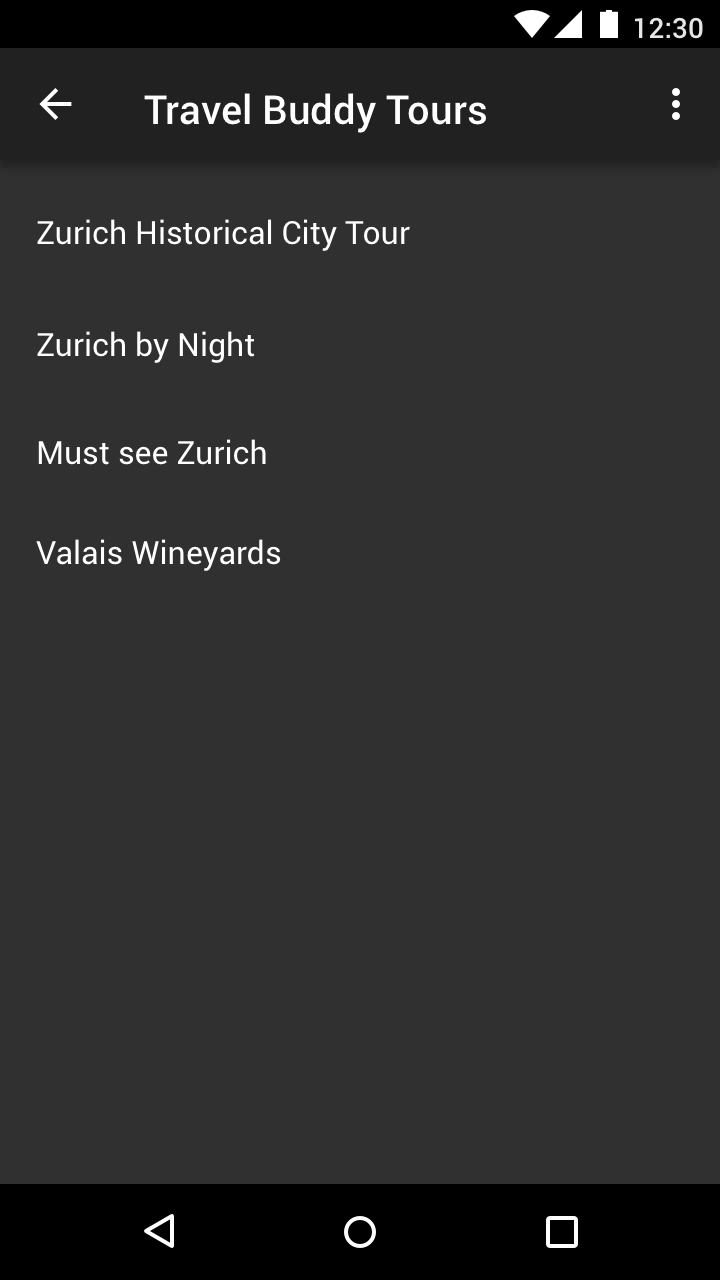
\includegraphics[width=\textwidth]{ListActivity}
    \caption{Startbildschirm von TravelBuddy}
  \end{minipage}
  \hfill
  \begin{minipage}[b]{0.48\textwidth}
    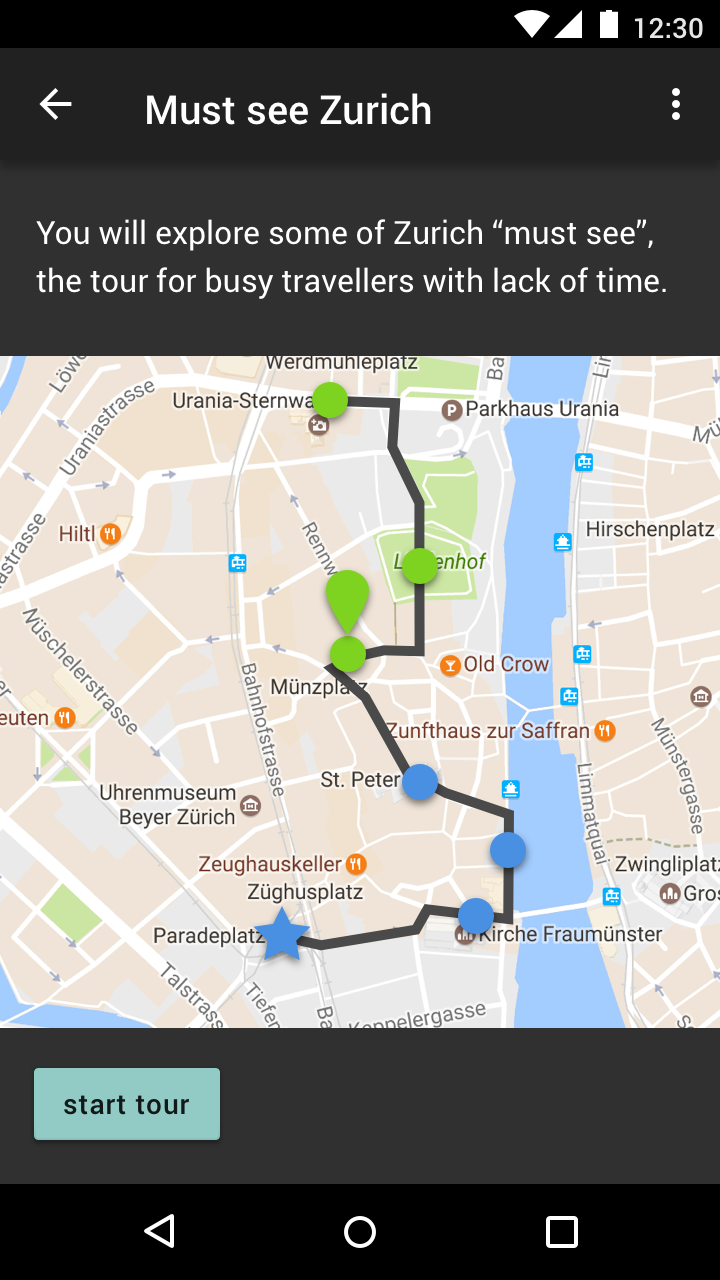
\includegraphics[width=\textwidth]{DetailActivity}
    \caption{Detailansicht einer Tour}
  \end{minipage}
\end{figure}

% TODO screenshot List & Detail activity

\subsection{Tour starten}

Sobald du eine Tour angetippt hast, erscheint zuunterst ein Knopf ``Tour starten''
mitwelchem du die Tour startest. Dir wird nun die Route zum ersten Wegpunkt angezeigt.
Begib dich nun auf den Weg zum ersten Punkt.

\begin{figure}
  \centering
  \begin{minipage}[b]{0.48\textwidth}
    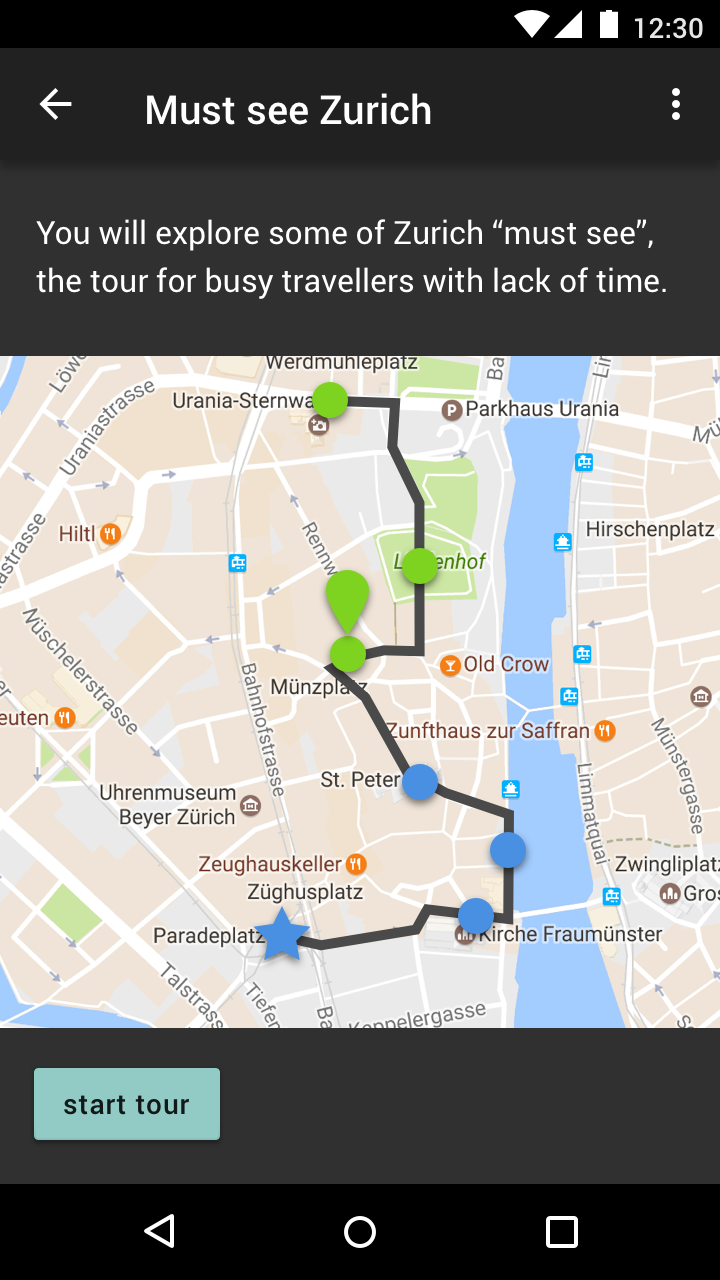
\includegraphics[width=\textwidth]{DetailActivity}
    \caption{Detailansicht einer Tour}
  \end{minipage}
  \hfill
  \begin{minipage}[b]{0.48\textwidth}
    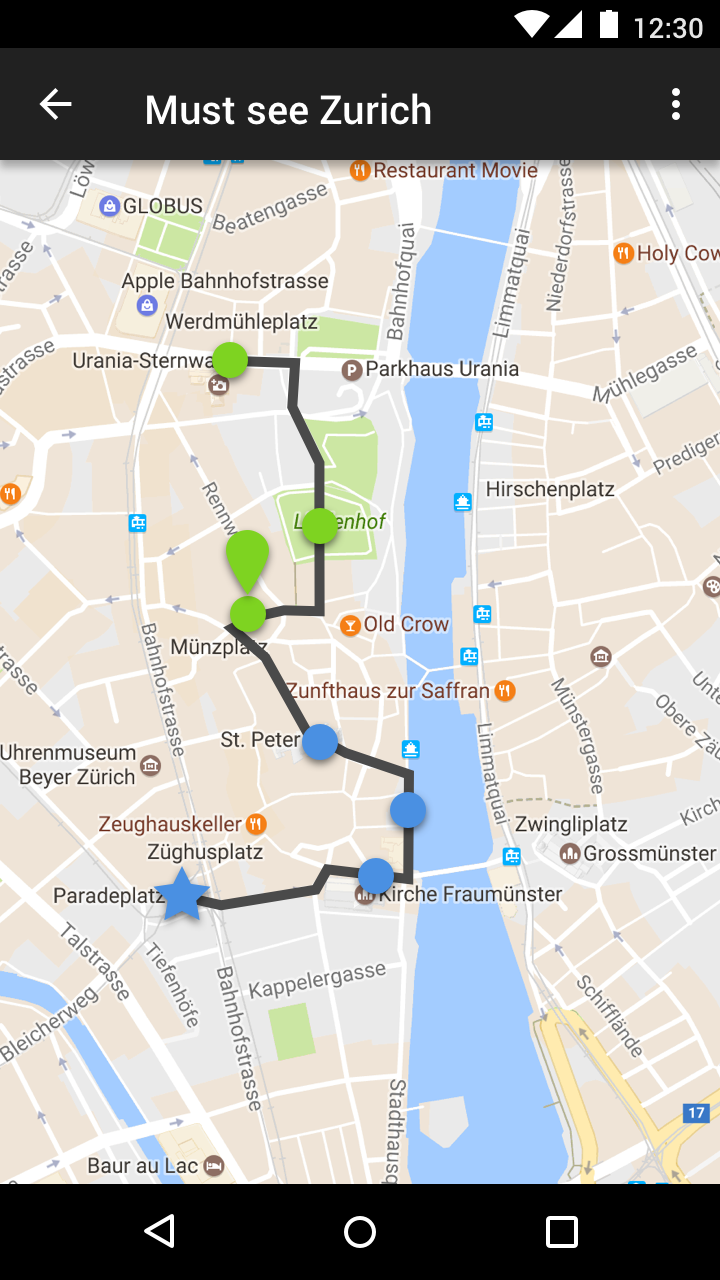
\includegraphics[width=\textwidth]{TourActivity}
    \caption{Route zum ersten Wegpunkt deiner Tour}
  \end{minipage}
\end{figure}

% TODO screenshot route activity > route
% TODO mention how to cancel a tour

\newpage
\subsection{Wegpunkt erreichen}

\begin{wrapfigure}{l}{0.5\textwidth}
  \begin{center}
    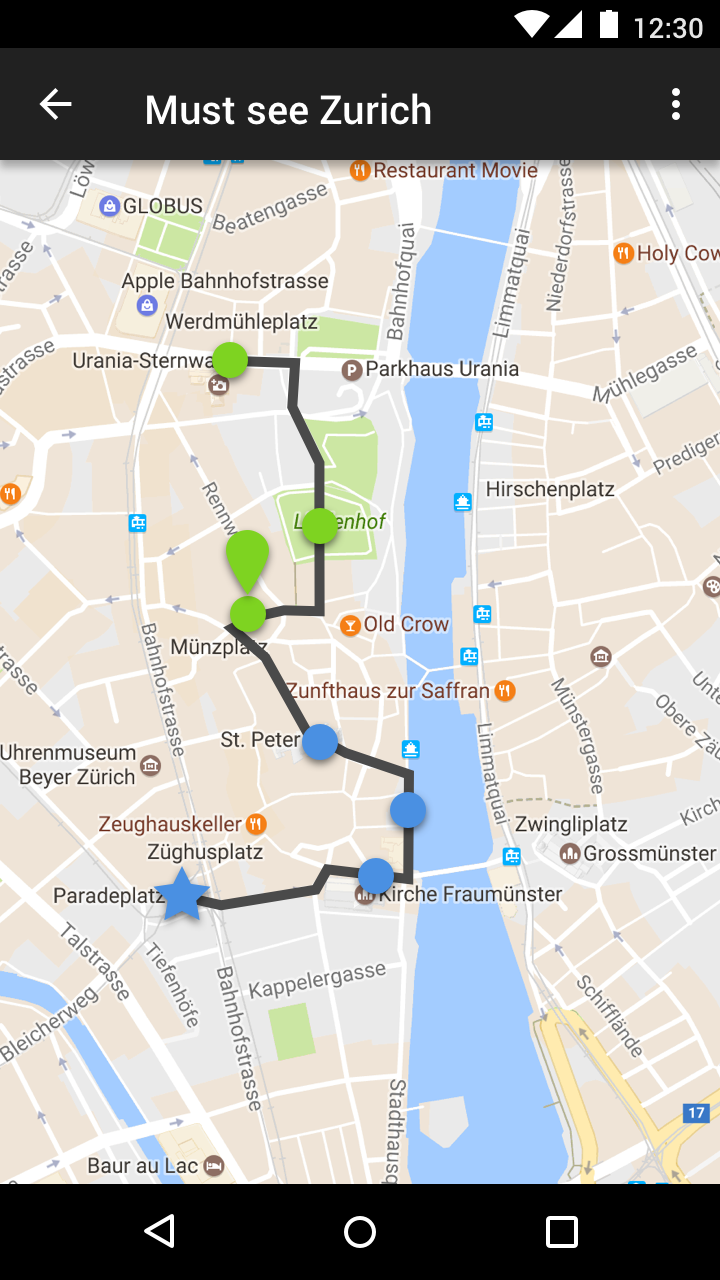
\includegraphics[width=0.48\textwidth]{TourActivity}
    \caption{Anzeige beim erreichen eines Wegpunktes}
  \end{center}
\end{wrapfigure}

Sobald du den Wegpunkt erreicht hast, zeigt dir TravelBuddy ein Foto von einer
Sehenswürdigkeit an. Schiesse nun ein Foto und tippe auf ``Foto überprüfen''.
Stimmt dein Foto mit dem Angezeigten überein, wird dir eine neue Route zum nächsten Punkt
angezeigt. Falls dein Foto nicht akzeptiert wird, nähere dich der Sehenswürdigtkeit auf dem
gezeigten Foto etwas und versuche es erneut.

% TODO screenshot route activity > picture
% TODO verify erbenjos

\newpage
\subsection{Tour abschliessen}
Sobald du den letzten Wegpunkt deiner Tour erreicht hast, zeigt dir TravelBuddy eine
Übersicht über deine gesamte Tour an. Du hast nun die Möglichkeit deine Fotos und einen
Überblick über deine Tour auf den sozialen Medien zu teilen. Tippe dafür einfach den
Knopf deines Netzwerkes an.

Sobald du auf ``Tour beenden'' tippst, gelangst du wieder auf den Startbildschirm von TravelBuddy.

\begin{wrapfigure}{l}{0.5\textwidth}
  \begin{center}
    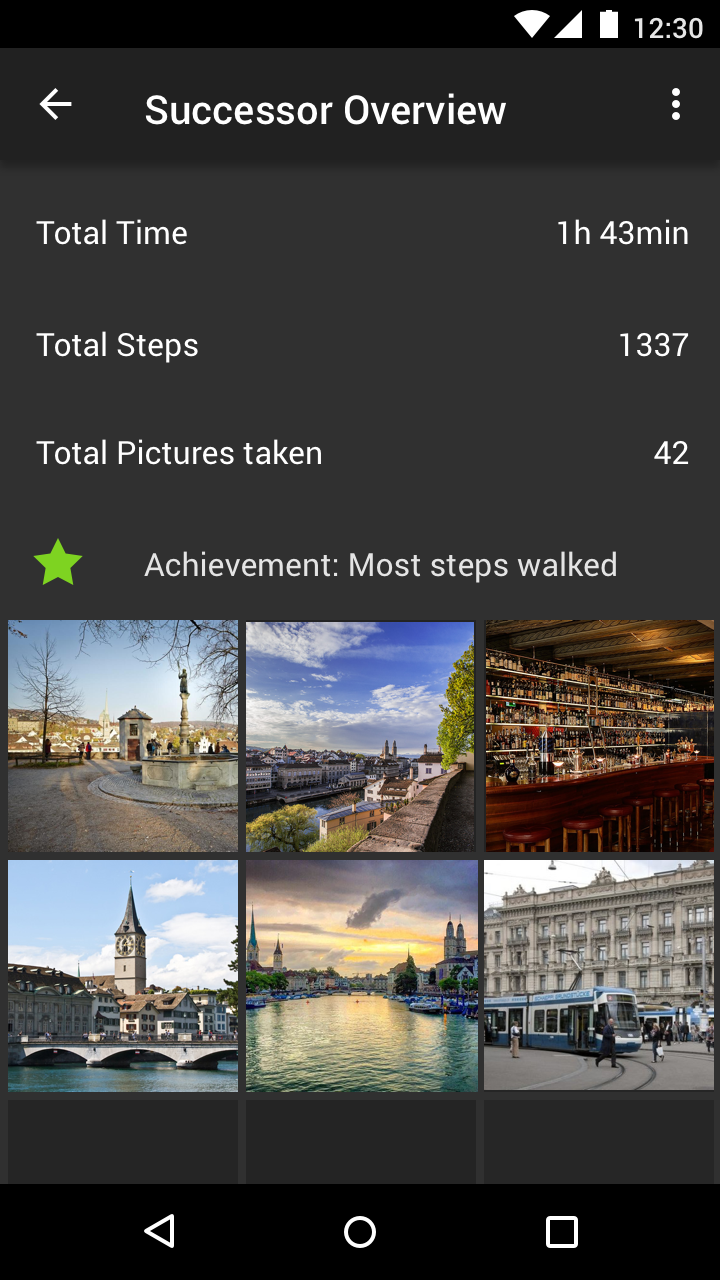
\includegraphics[width=0.48\textwidth]{SummaryActivity}
    \caption{Übersicht über deine Tour}
  \end{center}
\end{wrapfigure}

% TODO screenshot summary activity
% TODO verify bofraf
\end{document}
